\documentclass[a4paper,10pt]{article}
\usepackage[utf8]{inputenc}
\usepackage[spanish]{babel}
\usepackage{fancyhdr}
\usepackage{multicol}
\usepackage{geometry}
\usepackage{graphicx}
\usepackage{listings} 
\usepackage{xcolor} 
\geometry{a4paper, portrait, margin=1in}

\pagestyle{fancy}
\fancyhf{}
\fancyhead[L]{\textbf{Estadística Computacional}}
\fancyhead[R]{Universidad Nacional del Altiplano - FINESI}
\fancyfoot[C]{\thepage}

\lstset{
  backgroundcolor=\color{gray!10},
  basicstyle=\footnotesize\ttfamily,
  keywordstyle=\color{blue},
  commentstyle=\color{gray},
  stringstyle=\color{orange},
  frame=single,
  breaklines=true,
  showstringspaces=false
}

\begin{document}
\thispagestyle{fancy}

\begin{center}
    \textbf{\LARGE Análisis de regresión con datos del INEI usando Python y Optuna} \\
    \vspace{0.3cm}
    \textbf{Estudiante:} Mamani Huatta Cliver Daniel \\
    \textbf{Curso:} Estadística Computacional \\
    \textbf{Docente:} Torres Cruz Fred \\
    \textbf{Fecha:} 28 de mayo del 2025
\end{center}

\vspace{0.5cm}

\section*{Contextualización del Dataset y Aplicación de Regresión con Optuna}

Para la presente actividad se seleccionó un dataset real del Instituto Nacional de Estadística e Informática del Perú (INEI), correspondiente a la proyección de la población peruana para el año 2021. Este dataset incluye información desagregada por departamento, provincia, distrito, sexo y grupos de edad. La fuente es confiable, pública y ampliamente utilizada para la planificación de políticas públicas y estudios poblacionales. Para esta tarea se extrajo la información correspondiente a las edades y la cantidad de personas asociadas a cada grupo etario, con el objetivo de analizar su comportamiento.

La finalidad de utilizar este dataset fue predecir la cantidad de personas según la edad promedio. En otras palabras, se quiso estimar cuántas personas existen en cada grupo de edad utilizando modelos de regresión. Esta aplicación tiene utilidad real, por ejemplo, para la toma de decisiones en salud pública (planificación de vacunas, servicios de salud por edad), educación o pensiones.

\section*{Desarrollo del Modelo de Regresión}

El primer paso fue la preparación de los datos: se transformaron los rangos de edad (como ``65-69'') a un valor promedio (por ejemplo, 67), y se agrupó la información total de personas por edad. Luego se separaron los datos en conjuntos de entrenamiento y prueba.

Posteriormente, se implementó un modelo de regresión lineal utilizando la librería \texttt{scikit-learn}. Este modelo fue entrenado con los datos de edad como variable independiente (X) y la cantidad de personas como variable dependiente (y). La salida del modelo fue graficada para visualizar la relación entre ambas variables y la capacidad predictiva de la línea generada.

\begin{center}
    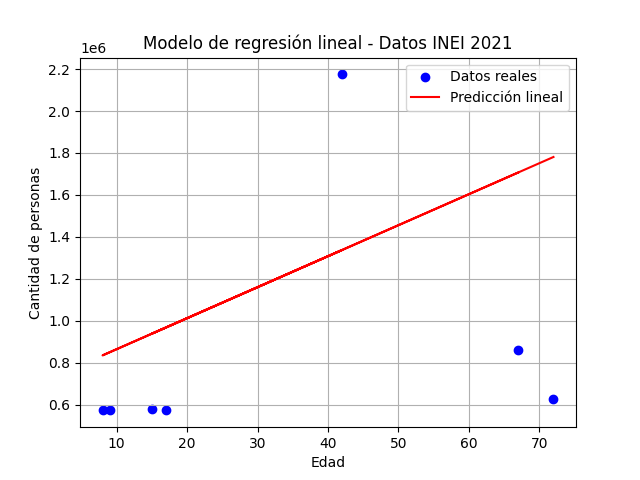
\includegraphics[width=0.75\textwidth]{DatosINEI.png} \\
    \small Figura 1: Gráfico de regresión lineal edad vs cantidad.
\end{center}

\section*{Comparación de Modelos con LazyPredict}

Con el objetivo de evaluar si existía un modelo mejor que la regresión lineal, se utilizó la librería \texttt{lazypredict}, que permite comparar automáticamente más de 30 modelos de regresión distintos. El resultado mostró que modelos como \texttt{ExtraTreesRegressor} y \texttt{RandomForestRegressor} superaban a la regresión lineal en términos del coeficiente de determinación (R2) y del error cuadrático medio (RMSE).

\section*{Optimización del Mejor Modelo con Optuna}

Tras identificar a \texttt{RandomForestRegressor} como uno de los modelos más prometedores, se procedió a optimizar sus hiperparámetros utilizando \texttt{Optuna}, una herramienta de optimización bayesiana. Se definieron los rangos de prueba para parámetros como la cantidad de árboles (\texttt{n\_estimators}), la profundidad máxima (\texttt{max\_depth}) y los mínimos requerimientos para dividir nodos (\texttt{min\_samples\_split}, \texttt{min\_samples\_leaf}).

Optuna realizó 30 intentos (trials) y determinó que la mejor combinación de hiperparámetros era: \texttt{n\_estimators=274}, \texttt{max\_depth=6}, \texttt{min\_samples\_split=2}, \texttt{min\_samples\_leaf=1}. Con estos parámetros, el modelo obtuvo un RMSE final de aproximadamente 109,979, lo cual representa un buen rendimiento para este tipo de datos poblacionales agregados.

\section*{Fragmento del Código en Python}

\begin{lstlisting}[language=Python]
import pandas as pd
import numpy as np
from sklearn.model_selection import train_test_split
from sklearn.linear_model import LinearRegression
from sklearn.ensemble import RandomForestRegressor
from sklearn.metrics import mean_squared_error
from lazypredict.Supervised import LazyRegressor
import matplotlib.pyplot as plt
import optuna

# 1. Leer el archivo CSV con los datos del INEI
datos = pd.read_csv("TB_POBLACION_INEI.csv", sep=';', encoding='latin1')
datos.columns = datos.columns.str.strip()

# 2. Convertir las edades de tipo rango a un número promedio
def promedio_edad(edad):
    if '-' in str(edad):
        partes = edad.split('-')
        return (int(partes[0]) + int(partes[1])) / 2
    try:
        return int(edad)
    except:
        return np.nan

datos['Edad'] = datos['Edad_Anio'].apply(promedio_edad)
datos['Cantidad'] = pd.to_numeric(datos['Cantidad'], errors='coerce')
datos = datos.dropna(subset=['Edad', 'Cantidad'])

# 3. Agrupar por edad para obtener la suma total por grupo
agrupado = datos.groupby('Edad')['Cantidad'].sum().reset_index()

# 4. Separar en datos de entrenamiento y prueba
X = agrupado[['Edad']]
y = agrupado['Cantidad']
X_entrenamiento, X_prueba, y_entrenamiento, y_prueba = train_test_split(X, y, test_size=0.2, random_state=42)

# 5. Modelo de regresión lineal
modelo_lineal = LinearRegression()
modelo_lineal.fit(X_entrenamiento, y_entrenamiento)
predicciones_lineal = modelo_lineal.predict(X_prueba)

# 6. Comparación de modelos con LazyPredict
comparador = LazyRegressor(verbose=0, ignore_warnings=True)
resultados, _ = comparador.fit(X_entrenamiento, X_prueba, y_entrenamiento, y_prueba)
print("Comparación de modelos regresivos:")
print(resultados)

# 7. Gráfico de la regresión lineal
plt.scatter(X_prueba, y_prueba, color='blue', label='Datos reales')
plt.plot(X_prueba, predicciones_lineal, color='red', label='Predicción lineal')
plt.xlabel('Edad')
plt.ylabel('Cantidad de personas')
plt.title('Modelo de regresión lineal - Datos INEI 2021')
plt.legend()
plt.grid(True)
plt.show()

# 8. Optimización de RandomForest usando Optuna
def funcion_objetivo(trial):
    arboles = trial.suggest_int("n_estimators", 10, 300)
    profundidad = trial.suggest_int("max_depth", 2, 20)
    division_minima = trial.suggest_int("min_samples_split", 2, 10)
    hojas_minimas = trial.suggest_int("min_samples_leaf", 1, 10)

    modelo = RandomForestRegressor(
        n_estimators=arboles,
        max_depth=profundidad,
        min_samples_split=division_minima,
        min_samples_leaf=hojas_minimas,
        random_state=42
    )
    modelo.fit(X_entrenamiento, y_entrenamiento)
    predicciones = modelo.predict(X_prueba)
    error_rmse = mean_squared_error(y_prueba, predicciones) ** 0.5
    return error_rmse

# Ejecutar la búsqueda de parámetros óptimos
estudio = optuna.create_study(direction="minimize")
estudio.optimize(funcion_objetivo, n_trials=30)

# Mostrar los mejores parámetros encontrados
print("\nMejores parámetros encontrados:")
print(estudio.best_params)

# Evaluar el modelo final con los parámetros óptimos
modelo_final = RandomForestRegressor(**estudio.best_params, random_state=42)
modelo_final.fit(X_entrenamiento, y_entrenamiento)
pred_final = modelo_final.predict(X_prueba)
rmse_final = mean_squared_error(y_prueba, pred_final) ** 0.5

print(f"\nError RMSE del modelo optimizado: {rmse_final:.2f}")
\end{lstlisting}

\section*{Conclusión}

En resumen, se logró contextualizar un dataset del INEI para aplicar técnicas de regresión, comparar distintos modelos y optimizar el más adecuado mediante Optuna. Esta experiencia permitió integrar conocimientos de preprocesamiento de datos, modelado predictivo, visualización y ajuste automático de hiperparámetros. 

Este trabajo me ayudó a entender mejor cómo aplicar modelos de regresión a datos reales y a automatizar la búsqueda de los mejores resultados con herramientas como Optuna.

\end{document}